\documentclass[letterpaper,10pt,draftclsnofoot,onecolumn]{IEEEtran}

\usepackage{graphicx}                                        
\usepackage{amssymb}                                         
\usepackage{amsmath}                                         
\usepackage{amsthm}                                          

\usepackage{alltt}                                           
\usepackage{float}
\usepackage{color}
\usepackage{url}

\usepackage{balance}
\usepackage[TABBOTCAP, tight]{subfigure}
\usepackage{enumitem}
\usepackage{pstricks, pst-node}

\usepackage{geometry}
\geometry{textheight=8.5in, textwidth=6in, margin=0.75in}

\usepackage{listings}
\lstset{ %
   language=C,                   % choose the language of the code
   basicstyle=\small,              % the size of the fonts that are used for the code
   keywordstyle=\color{blue},
   stringstyle=\color{cyan},
   commentstyle=\color{green},
   numbers=left,                   % where to put the line-numbers
   numberstyle=\footnotesize,      % the size of the fonts that are used for the line-numbers
   stepnumber=1,                   % the step between two line-numbers. If it is 1 each line will be numbered
   numbersep=5pt,                  % how far the line-numbers are from the code
   backgroundcolor=\color{white},  % choose the background color. You must add \usepackage{color}
   showspaces=false,               % show spaces adding particular underscores
   showstringspaces=false,         % underline spaces within strings
   showtabs=false,                 % show tabs within strings adding particular underscores
   frame=single,           		   % adds a frame around the code
   tabsize=2,          			   % sets default tabsize to 2 spaces
   captionpos=b,           		   % sets the caption-position to bottom
   breaklines=true,        		   % sets automatic line breaking
   breakatwhitespace=false,        % sets if automatic breaks should only happen at whitespace
   escapeinside={\%*}{*)}          % if you want to add a comment within your code
   }

%random comment

\newcommand{\cred}[1]{{\color{red}#1}}
\newcommand{\cblue}[1]{{\color{blue}#1}}

\usepackage{hyperref}
\usepackage{geometry}
\title{Team 11-06 Homework 2}
\def\name{Alex Wood, Miles Van de Wetering, Arman Hastings}

%pull in the necessary preamble matter for pygments output
%\input{pygments.tex}

%% The following metadata will show up in the PDF properties
\hypersetup{
  colorlinks = true,
  urlcolor = black,
  pdfauthor = {\name},
  pdfkeywords = {cs311 ``operating systems'' files filesystem I/O},
  pdftitle = {CS 311 Project 1: UNIX File I/O},
  pdfsubject = {CS 311 Project 1},
  pdfpagemode = UseNone
}

\begin{document}

\begin{titlepage}
   \centering
	{\scshape\Large Homework 2\par}
	\vspace{1.5cm}
	{\huge\bfseries CS 444 Spring 2017 Team 11-06\par}
	\vspace{2cm}
	{\Large\itshape \name \par}
    
    \date{\today}
    
    \vspace{2cm}
    
    \begin{abstract}
 	This is the report for group 11-06's homework 2. Homework 2 tasks teams with developing a patch for the Linux kernel which will contain a scheduler based on the noop scheduler, that implements a LOOK or C-LOOK scheduler. Once this is done, it is up to the teams to figure out how to apply and use the aforementioned patch. In addition to the primary assignment, a concurrency assignment was assigned which asked teams to create a solution to the Dining Philosophers problem.
   \end{abstract}
      
\end{titlepage}

\tableofcontents

\newpage

\section{Assignment Description}
This weeks kernel assignment is to implement a LOOK I/O scheduler for the Linux Yocto kernel. In this assignment we are to use the noop-iosched.c as a skeleton for implementing our scheduler patch. The noop-iosched is a FIFO scheduler with the proper structure for creating a scheduler. There are 3 functions that we will modify to accomplish the task of implementing the LOOK scheduler. We will utilize the power of the built-in 'elevator' algorithm implemented by the kernel designers. Our implementation will differ from the existing noop scheduler primarily because we will use an insertion sort to build and maintain our priority queue. 

The dining philosopher problem is designed to help students understand how to service multiple threads of a single process while maintaining proper shared memory management, and ensuring all threads are serviced.

\section{Design of SSTF Algorithm}
We decided to implement the LOOK algorithm for our scheduler. A LOOK scheduler that operates in both directions just seemed to make sense since the implementation doesn't add much complexity to the code. In order to accommodate this method of scheduling we created a function called find\_next, which uses the direction of the read head to determine where to insert the new request into the appropriate queue.
\begin{lstlisting}
static struct request* find_next(struct request_queue *q, struct sstf_data *nd) {
                struct request *entry;
		struct list_head *ptr;
		int found = 0;
		if(nd->direction == 1) {
                        list_for_each(ptr, &nd->queue) {
                                entry = list_entry(ptr, struct request, queuelist);
                                if(entry->bio->bi_iter.bi_sector > nd->last_dispatched) {
                                        found = 1;
                                        break;
                                }
                        }
                } else {
                        list_for_each_prev(ptr, &nd->queue) {
                                entry = list_entry(ptr, struct request, queuelist);
                                if(entry->bio->bi_iter.bi_sector < nd->last_dispatched) {
                                        found = 1;
                                        break;
                                }
                        }
                }
                if(found) {
                        nd->last_dispatched=entry->bio->bi_iter.bi_sector;
                        return entry;
                }
                else return NULL;
\end{lstlisting}
This function is used in conjunction with the sstf\_dispatch function. The dispatch function takes advantage of the functions built into the elevator algorithm found in elevator.h header file. Once a request is dispatched for execution, the function will output a printk statement indicating the current sector and whether it was a read or write operation.

Next, we modified the sstf\_add\_request function. This function, as with the dispatch function, was based directly off of the noop-iosched implementation and modified to implement the LOOK scheduler behavior. In order to get the noop-iosched to behave in this manner, we needed to make sure that the add request operation added the request to the proper sorted location based on the location of the read/write head and the location where the request data is to be read from or written too. This function ensures a sorted list, thus allowing us to be able to easily service requests in both directions of travel of the read head.

Lastly, to support all of these functions, we added two pieces of data to the sstf\_data struct - namely, direction (0|1) and last\_dispatched, which contained the sector of the most recent dispatched request. 

\section{Testing and Verification}

In order to test the application  we wrote a python script to generate a large amount of random I\textbackslash O. While this random I\textbackslash O is executed we pipe the output of the console to "tee" and store it in a file called output.txt. This will give use the current operations location on the "drive head". If this scheduler was implemented correctly we should see a graph that looks like a sawtooth pattern. 

After running several iterations of the test script on our scheduler implementation we saw strange behavior. Although we implemented a LOOK scheduler, the appearance of the first graph we saw made it appear to work like C-LOOK. As you can see in figure 1, the graph appears to show C-LOOK behavior through the majority of the run. 

\begin{figure}[!ht]
  \centering
  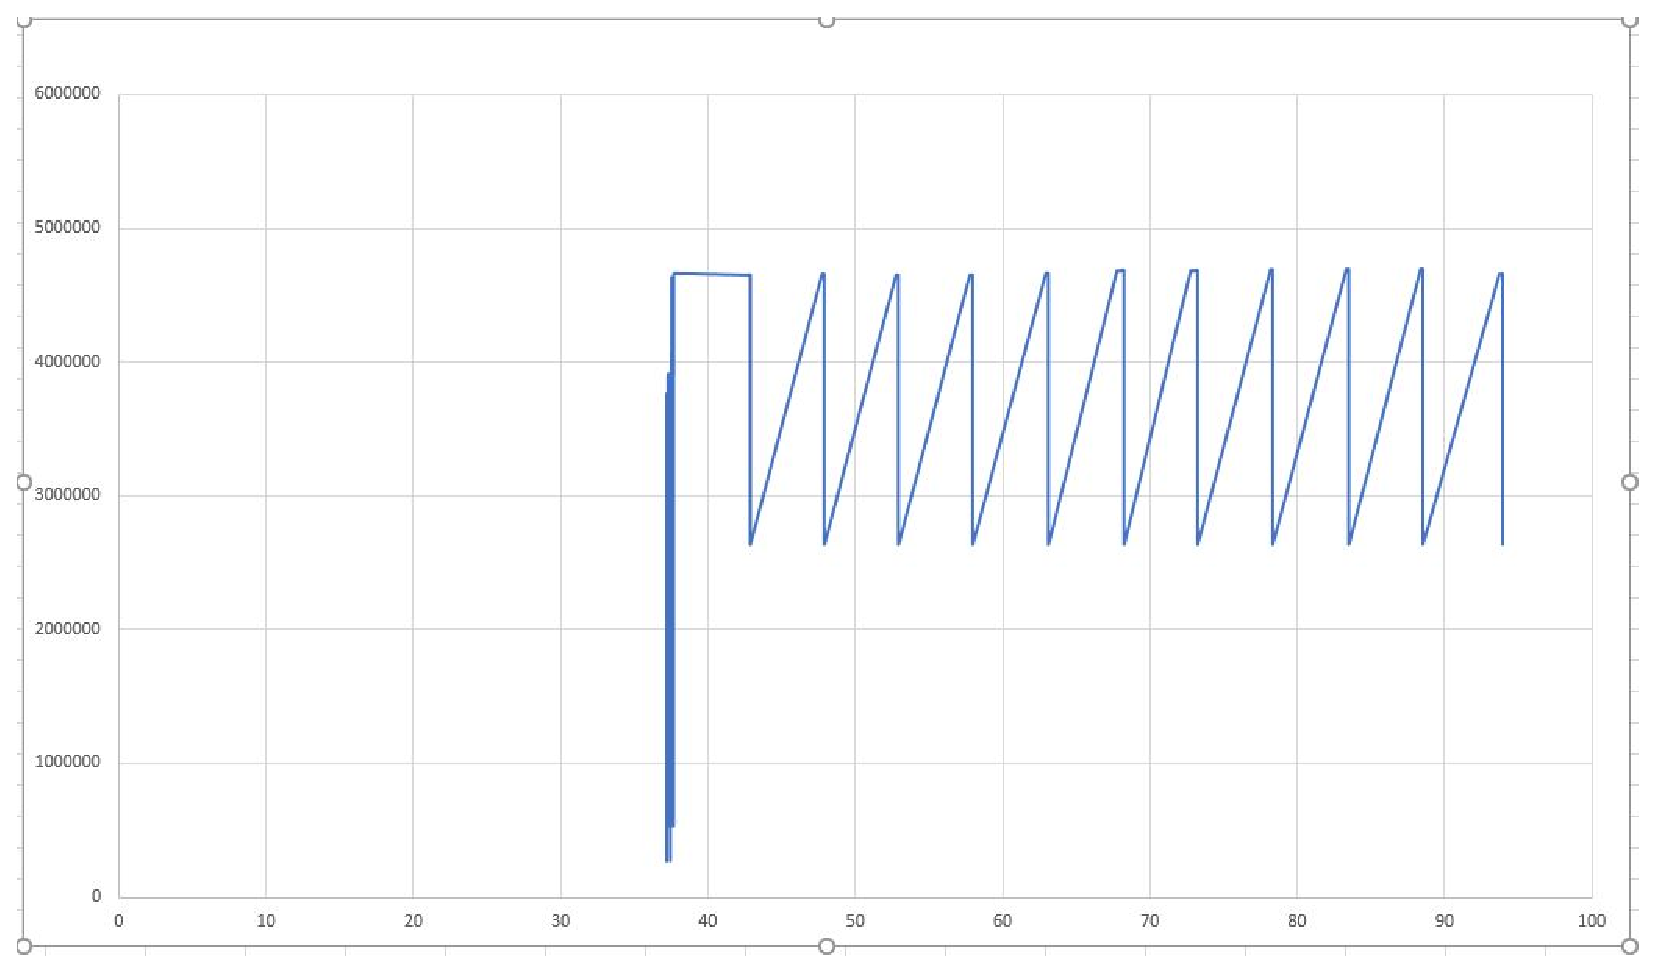
\includegraphics[width=1.0\textwidth]{CLOOK-Graph.eps}
  \centering
  \caption{The first graph from the first output test which indicates a CLOOK scheduler}
\end{figure}

It took several test runs before we decided to scale the x-axis to see what was happening in that first few milliseconds of our scheduler runs. In figure 2 you will see a later test in which we noticed there was something going on in the first section of the graph. We decided to zoom in to see what was happening in that section. 
\begin{figure}[!ht]
  \centering
  \includegraphics[width=1.0\textwidth]{graphComplete.eps}
  \centering
  \caption{A plot of our scheduler with 1720 random reads or writes.}
\end{figure}

In figure three you see a zoomed in section of the beginning of the graph of figure two. We theorize that this initial behavior is random because of the blocking nature of the I/O performed in our python script. After the script ran for some time, the files grew to a size large enough that the file system needed to move them around to keep them contiguous, which resulted in actually showing the appropriate CLOOK behavior. We are unsure why our code runs CLOOK instead of LOOK. 

\begin{figure}[!ht]
  \centering
  \includegraphics[width=1.0\textwidth]{graphFirstInt.eps}
  \centering
  \caption{First interval showing LOOK behavior}
\end{figure}

In figure four the pattern is still present.

\begin{figure}[!ht]
  \centering
  \includegraphics[width=1.0\textwidth]{graphSecondInt.eps}
  \centering
  \caption{Second interval showing LOOK behavior}
\end{figure}

In figure five you can see the randomness begin to show up. We believe this is due to the randomness of our testing script. 
\begin{figure}[ht!]
  \centering
  \includegraphics[width=1.0\textwidth]{graphThirdInt.eps}
  \centering
  \caption{The final interval in which the behavior switches to C-LOOK}
\end{figure}

After some period of time the file IO List is in order on the "disk", thus the insertions in essence create a FIFO. This behavior would change with the addition of more files to the list during the testing process. This verifies the operation of our scheduler.


\newpage

\section{Assignment 2 Report Questions}

\begin{enumerate}
\item What do you think the main point of this assignment is?

The point of this assignment was to get students to think about how IO is handled within the operating system. Although it did not take a large amount of code to complete this exercise, it took a lot of time to understand what it was we were trying to accomplish, what we needed to do to accomplish it, and what tools we had to be able to complete the task. 
\item How did you personally approach the problem? Design decisions, algorithm, etc.

Refer to section 2 as this was explained.

\item How did you ensure your solution was correct? Testing details, for instance.

See the Testing and Validation section above. 

\item What did you learn?

This assignment was able to give us a clearer picture of how an I\textbackslash O scheduler works in the Linux kernel, and by extension any scheduler in a general sense. There was a steep learning curve to this assignment. The code of the Linux kernel is intimidating to a novice, and this assignment forced us to get over that and to dig into a standard implementation of a Linux scheduler and to monkey with it to change its behavior. There are many parts of this assignment, that to our team, is new territory, which caused us to put in a significant amount of effort and thought into developing a solution. 
\end{enumerate}

\section{Work log}
\begin{tabular}{| p{2.1in} | p{2.3in} | p{2.1in} |}
\hline
Who & What & When \\
\hline
Alex, Arman, Miles & In recitation worked on the dining philosophers problem. Miles coded the assignment during class  & Recitation 11\\
\hline
Miles & Wrote code for a LOOK scheduler & May 2\\
\hline
Alex & Miles walked me through the code he created, and the functions he modified. Once I understood the code, I Went over code and made a couple of modifications to the printk() line. I added a priority and change the output a bit. Also Met with Arman about testing, after explaining the instructions, he began work on a python script to test the IO. & May2\\
\hline
Alex & Worked on getting the sstf scheduler loaded on the VM. Once loaded I created a python test script to test IO. Miles also created a python test script that was what was used for all the testing. Ran several tests of the scheduler with the python scripts, all of the kernel output was piped into tee to capture the output. Exported and graphed data & May 7\\
\hline
Miles & Wrote the patch for our scheduler, to convert from old files in linux/block to the new linux/block files & May 8\\
\hline
Alex and Miles & Worked together to get the the assignment all buttoned up. Staged all needed files for submission, tested makefile for the document submission, and all is working. We have a patch file, our Dining Philosopher concurrency assignment, and the patch file & May 8\\
\hline


\end{tabular}
%\bibliography{mybib}
%\bibliographystyle{ieeetr}

%\input{__mt19937ar.c.tex}

\end{document}